\documentclass[10pt]{article}
\usepackage[polish]{babel}
\usepackage[utf8]{inputenc}
\usepackage[T1]{fontenc}
\usepackage{amsmath}
\usepackage{amsfonts}
\usepackage{amssymb}
\usepackage[version=4]{mhchem}
\usepackage{stmaryrd}
\usepackage{graphicx}
\usepackage[export]{adjustbox}
\graphicspath{ {./images/} }

\title{KLASY PIERWSZE I DRUGIE }

\author{}
\date{}


\begin{document}
\maketitle
\begin{enumerate}
  \item Która liczba dwucyfrowa ma najwięcej dzielników?
  \item Wyznacz 10 ostatnich cyfr liczby 49! \(=1 \cdot 2 \cdot 3 \cdot \ldots \cdot 49\).
  \item Na okręgu o promieniu 1 opisano trójkąt prostokątny \(A B C\) o kącie prostym przy wierzchołku \(C\). Na przeciwprostokątnej \(A B\) tego trójkąta wybrano takie punkty \(D\) i \(E\), że zachodzą równości \(A D=A C\) i \(B E=B C\). Oblicz długość odcinka \(D E\).
\end{enumerate}

\section*{KLASY TRZECIE I CZWARTE}
\begin{enumerate}
  \item Dany jest trójkąt \(A B C\). Punkt I jest środkiem okręgu dopisanego do tego trójkąta stycznego do boku \(B C\), a punkty \(D\) iE to punkty styczności tego okręgu z przedłużeniami boków \(A B\) i AC. Punkt P to punkt przecięcia prostych DE i BI. Udowodnić, że kąt BPC jest prosty.
  \item W kwadracie \(A B C D\) wybieramy na boku \(B C\) taki punkt \(E\), a na boku \(C D\) taki punkt \(F\), że \(|E F|=|B E|+|F D|\). Udowodnij, że kąt \(E A F\) ma \(45^{\circ}\).
  \item Pole powierzchni wielościanu opisanego na kuli o promieniu 1 wynosi
  \item Oblicz objętość tego wielościanu.\\
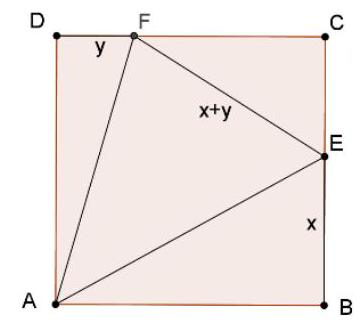
\includegraphics[max width=\textwidth, center]{2024_11_21_57e534bd5e068781e5c7g-1}
\end{enumerate}

\end{document}